\documentclass[a4paper,14pt]{extreport}

\usepackage{fontspec}
\setmainfont{XCharter}
%\setmainfont{CMU Serif}

\usepackage[none]{hyphenat}
\usepackage{graphicx}
\usepackage{subcaption}
\usepackage{hyperref}

\usepackage[bulgarian]{babel}
\usepackage{indentfirst}
%\setlength{\parindent}{0cm}

\usepackage[left=2cm,right=2cm,top=1cm,bottom=2cm]{geometry}

\usepackage{listings}
\lstset{
	language=c,
	basicstyle=\ttfamily\scriptsize,
	numbers=left,
}

\counterwithout{figure}{chapter}

%\usepackage{sectsty}
%\chapternumberfont{\Large}
%\chaptertitlefont{\huge}

\usepackage{schemabloc}
\usetikzlibrary{positioning}
\tikzset{%
  block/.style    = {draw, thick, rectangle, minimum height = 3em,
    minimum width = 10em},
}

\sloppy

\newcommand\pro{\item[$+$]}
\newcommand\con{\item[$-$]}

\begin{document}
\begin{titlepage}
	\centering
	{\scshape\LARGE Технологично училище\\„Електронни системи“ към\\Технически университет - София}
	\vfill
	{\scshape\LARGE Курсова работа} \\
	{\large Дистанционно за компютър}
	\vfill
	{
		Изготвил:        \hfill Преподавател: \\
		Теодор Тотев №20 \hfill Росен Витанов  \\
	}
	{\scshape\large София} \\
	{\large\the\year{} година}
\end{titlepage}

\chapter*{Увод}
\addcontentsline{toc}{chapter}{Увод}
Традиционно, хората се забавляват в домовете си чрез телевизори. До началото на двадесет и първи век
телевизорите имат достъп до малък брой аналогови канали, а след цифровизацията - до стотици. През
последните няколко години навлизат т. нар. „умни“ телевизори, позволяващи достъп до известни
стрийминг платформи.

Проектът дава на потребител възможността лесно да използва лаптопа си като телевизор посредством
\textit{дистанционно за компютър}. Този подход има много предимства пред умните телевизори:
възможността да се гледат свалени на диска видео файлове; възможността да се използват програми,
непредвидени от производител; премахване на нуждата за допълнително устройство; възможността да
продължи да се ползва по-стара техника.

Дистанционното позволява управление на курсора чрез променяне на посоката му. Подходът е избран пред
управлението чрез промяна в пространственото положение с оглед на ергономиата на проекта. Върху
дистанционното присъстват и често използвани копчета: ляво копче на мишката, дясно копче на
мишката, ескейп, цял екран, управление на звука, мултимедийно управление и прочие. Връзва се с
устройство с помощта на
безжична юесби шина.

\chapter{Вече съществуващи решения}
\section{W1 Air Mouse}

W1 Air Mouse продукт приближаващ се до изискванията на нашия проект. Представлява комбинация от
клавиатура и мишка. Използва акселерометър по три и жироскоп по три оси. Към него се отнасят
следните плюсове и минуси:

\begin{itemize}
	\pro Управление на курсора чрез посока на дистанционното.
	\pro Дълготрайна батерия.
	\pro Достъпна цена.
	\con Липсват копчета за мултимедийно управление.
	\con Клавиатурата лесно се натиска по неволя.
	\con Липсва подсветка на копчетата.
\end{itemize}

\begin{figure}[h]
	\centering
	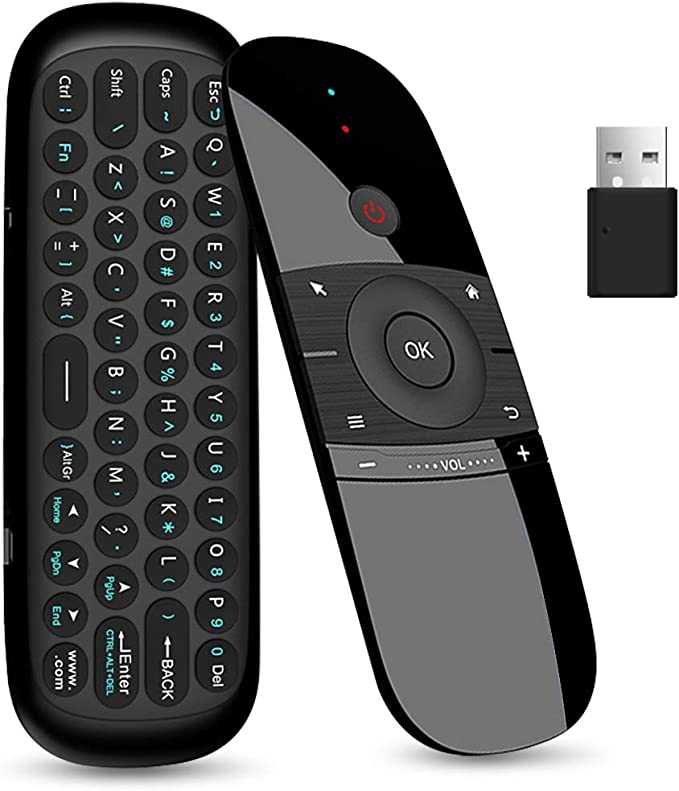
\includegraphics[width=0.25\textwidth]{w1-air-mouse}
	\caption{W1 Air Mouse}
\end{figure}

\section{Gimibox MX3 Pro}
Gimibox MX3 Pro продукт приближаващ се до изискванията на нашия проект. Представлява комбинация от
клавиатура и мишка. Използва акселерометър по три и жироскоп по три оси. Към него се отнасят
следните плюсове и минуси:
\begin{itemize}
	\pro Управление на курсора чрез посока на дистанционното.
	\pro Достъпна цена.
	\pro Изцяло може да замени дистанционното на обикновен телевизор.
	\con Липсва място за складиране на юесби шината.
	\con Краткотрайна батерия
	\con Липсва подсветка на копчетата.
\end{itemize}

\begin{figure}[h]
	\centering
	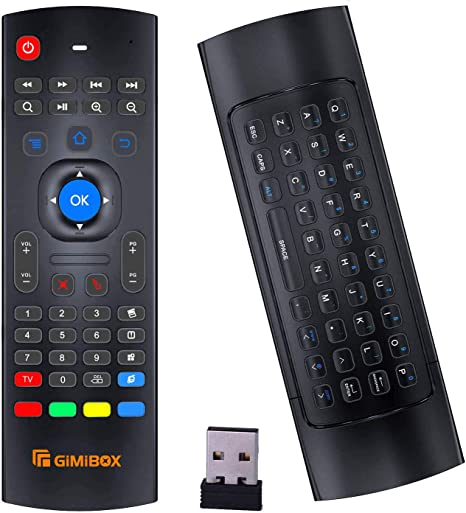
\includegraphics[width=0.25\textwidth]{gimbox-mx3-pro}
	\caption{W1 Air Mouse}
\end{figure}

\chapter{Структура на проекта}
\section{Обзор}
В основата на проекта седи Ардуино микро с ATmega32U4. То управлява сензори за жироскоп,
акселерометър и компас, които се използват за отчитане на посоката на дистанционното. Отчетените
данни се превеждат в движение на курсора. Дистанционното получава сигнал и от копчетата, разположени
върху него. Командите на потребителя се предават на компютъра посредством юесби шина. Комуникацията
по юесби се извършва с помощта на вградените в Ардуино библиотеки \textit{Mouse.h} и
\textit{Keyboard.h}. Проектът се захранва от две успоредно свързани литиевойонни
батерии.

\section{Подробен преглед}
Ардуино микро е микроконтролер, основан на чипа \textit{ATmega32U4}. Има двадесет цифрови
входно-изходни щифта, от които седем могат да бъдат използвани за изход в широчино-импулсна
модулация и дванадесет като аналогов вход. В ATmega32U4 е вградена юесби комуникация, позволяваща на
микро да се държи като клавиатура и мишка. Това му качество съчетано с малките му физически размери
го правят подходящ микроконтролер за проекта.

MPU6500 съчетава акселерометър и жироскоп в един чип. Чипът комуникира с микроконтролера посредством
I²C. Частта е избрана поради малките ѝ физически размери и достъпната ѝ цена.

За компас е избран HMC5883. Чипът комуникира с микроконтролера посредством I²C. Частта е избрана
поради малките ѝ физически размери и достъпната ѝ цена.

\begin{figure}[h]
	\centering
	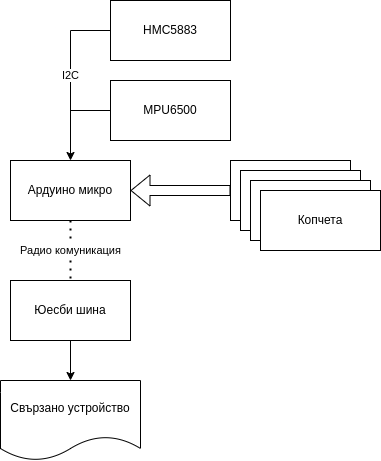
\includegraphics[width=1\textwidth]{block-scheme}
	\caption{Блок схема на проекта}
\end{figure}

\chapter*{Използвана литература}
\addcontentsline{toc}{chapter}{Използвана литература}
\url{https://docs.arduino.cc/hardware/micro} \\
\url{https://www.amazon.com/Android-Gimibox-Wireless-Keyboard-Projector/dp/B07WJGSXT8} \\
\url{https://www.amazon.com/Universal-Wireless-Keyboard-Connection-Projector/dp/B07WRZNW6X} \\

\tableofcontents
\end{document}
